\documentclass{beamer}
\mode<presentation>
\usepackage{amsmath}
\usepackage{amssymb}
%\usepackage{advdate}
\usepackage{adjustbox}
\usepackage{subcaption}
\usepackage{enumitem}
\usepackage{multicol}
\usepackage{mathtools}
\usepackage{listings}
\usepackage{url}
\def\UrlBreaks{\do\/\do-}
\usetheme{metropolis}
%\usecolortheme{lily}
\setbeamertemplate{footline}
{
  \leavevmode%
  \hbox{%
  \begin{beamercolorbox}[wd=\paperwidth,ht=2.25ex,dp=1ex,right]{author in head/foot}%
    \insertframenumber{} / \inserttotalframenumber\hspace*{2ex} 
  \end{beamercolorbox}}%
  \vskip0pt%
}
\setbeamertemplate{navigation symbols}{}

\providecommand{\nCr}[2]{\,^{#1}C_{#2}} % nCr
\providecommand{\nPr}[2]{\,^{#1}P_{#2}} % nPr
\providecommand{\mbf}{\mathbf}
\providecommand{\pr}[1]{\ensuremath{\Pr\left(#1\right)}}
\providecommand{\qfunc}[1]{\ensuremath{Q\left(#1\right)}}
\providecommand{\sbrak}[1]{\ensuremath{{}\left[#1\right]}}
\providecommand{\lsbrak}[1]{\ensuremath{{}\left[#1\right.}}
\providecommand{\rsbrak}[1]{\ensuremath{{}\left.#1\right]}}
\providecommand{\brak}[1]{\ensuremath{\left(#1\right)}}
\providecommand{\lbrak}[1]{\ensuremath{\left(#1\right.}}
\providecommand{\rbrak}[1]{\ensuremath{\left.#1\right)}}
\providecommand{\cbrak}[1]{\ensuremath{\left\{#1\right\}}}
\providecommand{\lcbrak}[1]{\ensuremath{\left\{#1\right.}}
\providecommand{\rcbrak}[1]{\ensuremath{\left.#1\right\}}}
\theoremstyle{remark}
\newtheorem{rem}{Remark}
\newcommand{\sgn}{\mathop{\mathrm{sgn}}}
\providecommand{\abs}[1]{\left\vert#1\right\vert}
\providecommand{\res}[1]{\Res\displaylimits_{#1}} 
\providecommand{\norm}[1]{\lVert#1\rVert}
\providecommand{\mtx}[1]{\mathbf{#1}}
\providecommand{\mean}[1]{E\left[ #1 \right]}
\providecommand{\fourier}{\overset{\mathcal{F}}{ \rightleftharpoons}}
%\providecommand{\hilbert}{\overset{\mathcal{H}}{ \rightleftharpoons}}
\providecommand{\system}{\overset{\mathcal{H}}{ \longleftrightarrow}}
	%\newcommand{\solution}[2]{\textbf{Solution:}{#1}}
%\newcommand{\solution}{\noindent \textbf{Solution: }}
\providecommand{\dec}[2]{\ensuremath{\overset{#1}{\underset{#2}{\gtrless}}}}
\newcommand{\myvec}[1]{\ensuremath{\begin{pmatrix}#1\end{pmatrix}}}
\let\vec\mathbf

\lstset{
%language=C,
frame=single, 
breaklines=true,
columns=fullflexible
}

\numberwithin{equation}{section}

\title{Computationally solving differential equations \brak{\text{9.1.3}}}
\author{Agamjot Singh,\\EE24BTECH11002,\\IIT Hyderabad.}

\date{\today} 
\begin{document}

\begin{frame}
\titlepage
\end{frame}

\section*{Outline}
\begin{frame}
\frametitle{Table of Contents}
\tableofcontents
\end{frame}

\section{Problem}

\begin{frame}
\frametitle{Problem Statement}
Solve the differential equation:
\begin{align}
    \frac{d^2 y}{d x^2} + y = 0
\end{align}
\end{frame}

\section{Solution}

%Slide1
\subsection{Theoretical Solution}
\begin{frame}
\frametitle{Theoretical Solution}
The given differential equation is a second-order linear ordinary differential equation. \newline
Let $y\brak{0} = c_1$ and $y^{\prime}\brak{0} = c_2$.
By definition of Laplace transform,
\begin{align}
    \mathcal{L}\brak{f\brak{t}} = \int_0^{\infty} e^{-st} f\brak{t} \, dt
\end{align}
Some used properties of Laplace transform include,
\begin{align}
    \mathcal{L}\brak{y^{\prime\prime}} &= s^2\mathcal{L}\brak{y} -sy\brak{0}-y^\prime\brak{0} = s^2\mathcal{L}\brak{y} -sc_1 - c_2\\
    \mathcal{L}\brak{\cos{t}} &= \frac{s}{s^2 + 1}\\
    \mathcal{L}\brak{\sin{t}} &= \frac{1}{s^2 + 1}\\
    \mathcal{L}\brak{cf\brak{t}} &= c\mathcal{L}\brak{f\brak{t}}\\
    \mathcal{L}\brak{f\brak{t}} &= F\brak{s} \implies \mathcal{L}\brak{e^{at}f\brak{t}} = F\brak{s-a}
\end{align}
\end{frame}

%Slide2
\begin{frame}
Applying Laplace transform on the given differential equation, we get,
\begin{align}
    y^{\prime\prime} + y &= 0\\
    \mathcal{L}\brak{y^{\prime\prime}} + \mathcal{L}\brak{y} &= 0\\
    s^2\mathcal{L}\brak{y} - sc_1 - c_2 + \mathcal{L}\brak{y} &= 0\\
    \mathcal{L}\brak{y} &= \frac{sc_1 + c_2}{s^2 + 1} = c_1\frac{s}{s^2 + 1} + c_2\frac{1}{s^2 + 1} \label{laplace_eq}
\end{align}
Taking laplace inverse on both sides, we get,
\begin{align}
    y &= c_1\mathcal{L}^{-1}\brak{\frac{s}{s^2 + 1}} + c_2\mathcal{L}^{-1}\brak{\frac{1}{s^2 + 1}}\\
    y &= c_1\cos{x} + c_2\sin{x}\\
    \implies y\brak{x} &= 
    \begin{cases}
        \sqrt{\brak{c_1}^2 + \brak{c_2}^2} \sin{\brak{x + \tan^{-1}{\brak{\frac{c_1}{c_2}}}}} & \quad c_2 \neq 0\\
        c_1\cos{x} & \quad c_2 = 0
    \end{cases}
\end{align}
\end{frame}

%Slide3
\subsection{Computation Solution - Trapezoid Method}
\begin{frame}
\frametitle{Computation Solution - Trapezoid Method}
The given differential equation can be represented as 
\begin{align}
    y^{\prime\prime} + y = 0
\end{align}
Let $y = y_1$ and $y^{\prime} = y_2$, then, 
\begin{align}
    \frac{dy_2}{dx} &= -y_1 \text{ and } \frac{dy_1}{dx} = y_2\\
    \int_{y_{2, n}}^{y_{2, n + 1}} \, dy_2 &= \int_{x_n}^{x_{n + 1}} -y_1 \, dx\\
    \int_{y_{1, n}}^{y_{1, n + 1}} \, dy_1 &= \int_{x_n}^{x_{n + 1}} y_2 \, dx\\
\end{align}
\end{frame}

%Slide4
\begin{frame}
Discretizing the steps \brak{\text{Trapezoid rule}},
\begin{align}
    y_{2, n + 1} - y_{2, n} &= -\frac{h}{2}\brak{y_{1, n} + y_{1, n + 1}}\\
    y_{1, n + 1} - y_{1, n} &= \frac{h}{2}\brak{y_{2, n} + y_{2, n + 1}}
\end{align}
Solving for $y_{1, n + 1}$ and $y_{2, n + 1}$, we get,
\begin{align}
    y_{1, n + 1} = y_{1, n} + \frac{h}{2}\brak{2y_{2, n} - \frac{h}{2}\brak{y_{1, n} + y_{1, n + 1}}}
\end{align}
The difference equations can be written as,
\begin{align}
    y_{1, n + 1} = \frac{\brak{4 - h^2}y_{1, n} + 4hy_{2, n}}{\brak{4 + h^2}}\\
    y_{2, n + 1} = \frac{\brak{4 - h^2}y_{2, n} - 4hy_{1, n}}{\brak{4 + h^2}}
\end{align}
\end{frame}

%Slide4
\begin{frame}
Iteratively plotting the above system taking intial conditions as 
\begin{align}
    x_0 = 0 \text{ , } y_{1, 0} = 0 \text{ , } y_{2, 0} = 1
\end{align}
we get the plot of the given differential equation.
\end{frame}

%Slide5
\subsection{Computation Solution - Bilinear Transform Method}
\begin{frame}
\frametitle{Computation Solution - Bilinear Transform Method}
We have to apply laplace transformation on the given differential equation. From \brak{\ref{laplace_eq}}, we get,
\begin{align}
    Y\brak{s} &= \frac{sc_1 + c_2}{s^2 + 1}
\end{align}
\begin{align}
    Y\brak{s} &= \frac{sc_1 + c_2}{s^2 + 1}
\end{align}
Applying Bilinear transform, with $T = h$, we get,
\begin{align}
    s &= \frac{2}{T}\frac{1 - z^{-1}}{1 + z^{-1}} = \frac{2}{h}\frac{1 - z^{-1}}{1 + z^{-1}}\\
    \implies Y\brak{z} &= \frac{2hc_1 \brak{z^2 - 1} + c_2h^2 \brak{z + 1}^2}{\brak{h^2 + 4}z^2 + 2\brak{h^2 - 4}z + \brak{h^2 + 4}}
\end{align}
\end{frame}

%Slide6
\begin{frame}
    Note that this transformation is stable only when the poles of $Y\brak{s}$ lie inside the unit circle centered at origin. The poles for the given $Y$ is $s = \pm i$ which both lie on $\abs{s} = 1$, thus this system is stable.
\begin{multline}
    \brak{z^2 + 2\frac{h^2 - 4}{h^2 + 4}z + 1} Y\brak{z} \\
    = \frac{2hc_1 \brak{z^2 - 1} + c_2h^2 \brak{z^2 + 2z + 1}}{h^2 + 4}
\end{multline}
\begin{multline}
    z^2Y\brak{z} + 2\frac{h^2 - 4}{h^2 + 4}zY\brak{z} + Y\brak{z} \\
    = \frac{\brak{2h c_1 + c_2 h^2}z^2 + \brak{2h^2 c_2}z + \brak{h^2c_2 - 2hc_1}}{h^2 + 4} \label{bilinear_eq}
\end{multline}
\end{frame}

%Slide7
\begin{frame}
Some properties of one sided $z$ transform,
\begin{align}
    \mathcal{Z}\brak{y\sbrak{n + 2}} &= z^2 Y\brak{z} - y\sbrak{1}z - y\sbrak{0}\\
    \mathcal{Z}\brak{y\sbrak{n + 1}} &= z Y\brak{z} - z y_\sbrak{0}\\
    \mathcal{Z}\brak{\delta\sbrak{n}} &= 1 \text{, } z \neq 0\\
    \mathcal{Z}\brak{y\sbrak{n}} = Y\brak{z} &\implies \mathcal{Z}\brak{y\sbrak{n - n_0}} = z^{-n_0}Y\brak{z} \label{time_shift_eq}
\end{align}
By the time shift property $\brak{\ref{time_shift_eq}}$,
\begin{align}
    \mathcal{Z}\brak{\delta\sbrak{n + 2}} &= z^2 \text{, } z \neq 0\\
    \mathcal{Z}\brak{\delta\sbrak{n + 1}} &= z \text{, } z \neq 0
\end{align}
\end{frame}

%Slide8
\begin{frame}
Rewriting equation $\brak{\ref{bilinear_eq}}$, we get,
\begin{align}
    &z^2Y\brak{z} + 2\frac{h^2 - 4}{h^2 + 4}zY\brak{z} + Y\brak{z} + \brak{- y\sbrak{1}z - y\sbrak{0}} \nonumber\\
    &+ 2\brak{\frac{h^2 - 4}{h^2 + 4}}\brak{-zy\sbrak{0}} = \frac{\brak{2h c_1 + c_2 h^2}z^2}{h^2 + 4} \nonumber\\
    &+ \frac{2h^2 c_2 - \brak{h^2 + 4}y\sbrak{1} - 2\brak{h^2 - 4}y\sbrak{0}}{h^2 + 4} \nonumber\\
    &+ \frac{z\brak{h^2c_2 - 2hc_1 - \brak{h^2 + 4}y\sbrak{0}}}{h^2 + 4} \label{z_trans_eq}\\
    &\text{where } z \neq 0
\end{align}
Region of convergence $\brak{\textbf{ROC}}$ is given by $z \neq 0$.
\end{frame}

%Slide9
\begin{frame}
Taking $z$ inverse transform on both sides of equation $\brak{\ref{z_trans_eq}}$, we get the $\textbf{difference equation}$ which is given by,
\begin{align}
    y&\sbrak{n + 2} + 2\brak{\frac{h^2 - 4}{h^2 + 4}} y\sbrak{n + 1} + y\sbrak{n} \nonumber\\
    &= \frac{\brak{2h c_1 + c_2 h^2}\delta\sbrak{n + 2}}{h^2 + 4} \nonumber\\
    &+ \frac{\brak{2h^2 c_2 - \brak{h^2 + 4}y\sbrak{1} - 2\brak{h^2 - 4}y\sbrak{0}}\delta\sbrak{n + 1}}{h^2 + 4} \nonumber\\
    &+ \frac{\brak{h^2c_2 - 2hc_1 - y\sbrak{0}}\delta\sbrak{n}}{h^2 + 4} \label{diff_eq}
\end{align}
Here, $\delta$ is given by,
\begin{align}
    \delta\sbrak{n - n_0} =
    \begin{cases}
        1 & \quad n = n_0\\
        0 & \quad n \neq n_0
    \end{cases}
\end{align}
\end{frame}

%Slide10
\begin{frame}
As $n > 0$, 
\begin{align}
    \delta\sbrak{n + 2} = \delta\sbrak{n + 1} = 0
\end{align}
The equation \brak{\ref{diff_eq}} is now given by,
\begin{align}
    y\sbrak{n + 2} + 2\brak{\frac{h^2 - 4}{h^2 + 4}} y\sbrak{n + 1} + y\sbrak{n} = \frac{\brak{h^2c_2 - 2hc_1 - y\sbrak{0}}\delta\sbrak{n}}{h^2 + 4} 
\end{align}
At this point we drop the notation $y\sbrak{n}$ and replace it with $y_n$, and we replace $c_1 = y\brak{0}$ and $c_2 = y^{\prime}\brak{0}$,
\begin{align}
    y_{n + 2} + 2\brak{\frac{h^2 - 4}{h^2 + 4}} y_{n + 1} + y_{n} = \frac{\brak{h^2y^{\prime}\brak{0} - 2hy\brak{0} - y_0}\delta\sbrak{n}}{h^2 + 4} 
\end{align}
\end{frame}

%Slide11
\begin{frame}
Note that for computationally plotting the above difference equation, we need $y_0 = y\brak{0}$ as well as $y_1$. To find $y_1 = y\brak{0 + h} = y\brak{h}$ we employ first principle of derivative,
\begin{align}
    y^{\prime}\brak{x} &= \lim_{h\to0} \frac{y\brak{x + h} - y\brak{x}}{h}\\
    y\brak{x + h} &= y\brak{x} + hy^{\prime}\brak{x}, h\to0\\
    y_1 &= y\brak{h} = y\brak{0} + hy^{\prime}\brak{0}
\end{align}

Iteratively plotting the above system taking intial conditions as 
\begin{align}
    x_0 = 0 \text{ , } y_{0} = y\brak{0} = 0 \text{ , } y^{\prime}\brak{0} = 1
\end{align}
we get the plot of the given differential equation.
\end{frame}

%Slide12
\subsection{Plot}
\begin{frame}
\frametitle{Plot}
\begin{figure}[h!]
   \centering
   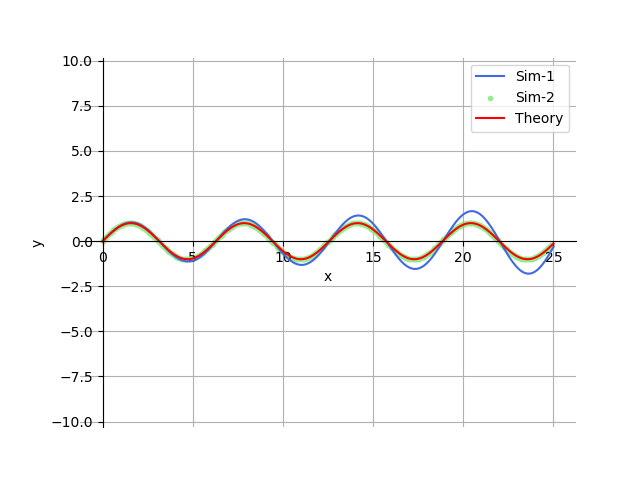
\includegraphics[width=0.7\linewidth]{figs/graph.png}
   \caption{Here Sim-$1$ plot represents the plot given by Trapezoid Method, and Sim-$2$ which is given by Bilinear transform using the same value of $h$. This plot clearly shows the accuracy of the Bilinear transform method.}
\end{figure}
\end{frame}

\end{document}
